%%%%%%%%%%%%%%%%%%%%%%%%%%%%%%%%%%%%%%%%%%%%%%%%%%%%%%%
% ultimate plantUML Cheatsheet
%
% Based on MatPlotLib Cheatsheet by Michelle Baltazar https://www.overleaf.com/latex/examples/matplotlib-and-random-cheat-sheet/yttxrcxntbht
%
%%%%%%%%%%%%%%%%%%%%%%%%%%%%%%%%%%%%%%%%%%%%%%%%%%%%%%%

\documentclass{article}
\usepackage[landscape]{geometry}
\usepackage{hyperref}
\usepackage{multicol}
\usepackage{amsfonts}
\usepackage{tikz}
\usetikzlibrary{decorations.pathmorphing}

\usepackage{colortbl}
\usepackage{xcolor}

\title{ultimate plantUML Cheatsheet}
\usepackage[utf8]{inputenc}

\advance\topmargin-.8in
\advance\textheight3in
\advance\textwidth3in
\advance\oddsidemargin-1.5in
\advance\evensidemargin-1.5in
\parindent0pt
\parskip2pt
\newcommand{\hr}{\centerline{\rule{3.5in}{1pt}}}
%\colorbox[HTML]{e4e4e4}{\makebox[\textwidth-2\fboxsep][l]{texto}
\begin{document}

\begin{center}{\huge{\textbf{ultimate plantUML Cheatsheet}}}\\
{\large by \href{http://anoff.io}{Andreas Offenhaeuser}}
\end{center}
\begin{multicols*}{3}

\tikzstyle{mybox} = [draw=black, fill=white, very thick,
    rectangle, rounded corners, inner sep=10pt, inner ysep=10pt]
\tikzstyle{fancytitle} =[fill=black, text=white, font=\bfseries]

\newcommand{\block}[2]{%
  \begin{tikzpicture}%
  \node [mybox] (box){%
    \begin{minipage}{0.3\textwidth}%
		#2%
    \end{minipage}%
  };%
\node[fancytitle, right=10pt] at (box.north west) {#1};
\end{tikzpicture}%
}

\block{Components}{

  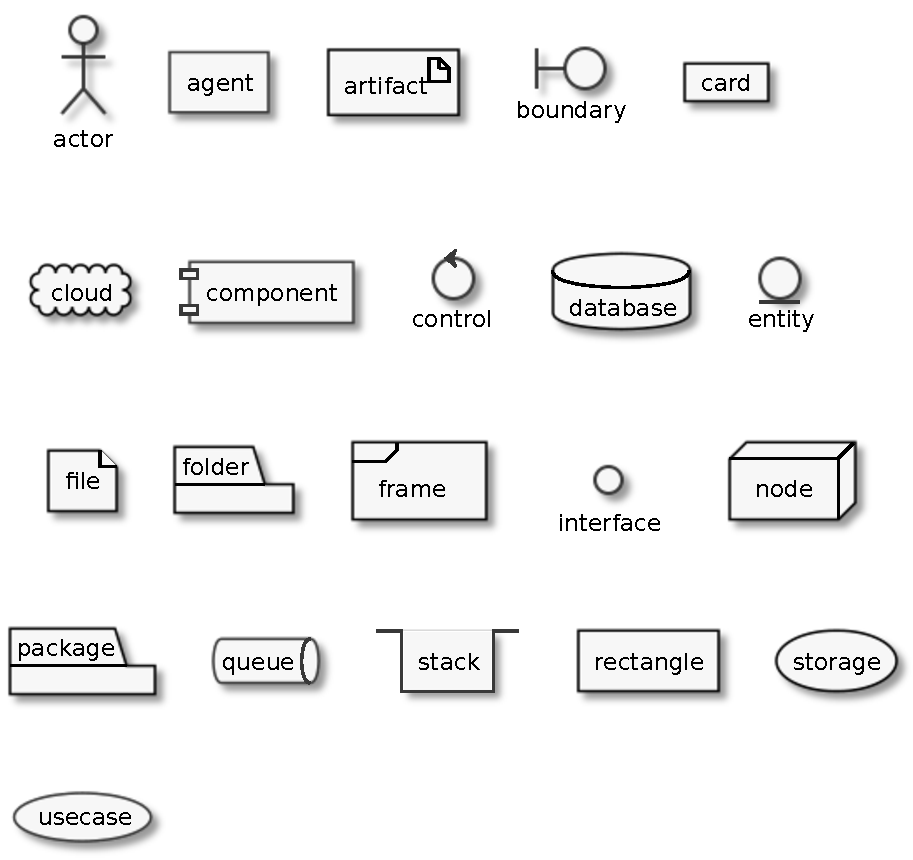
\includegraphics[width=\textwidth]{diagrams/dist/components.pdf} 
}

\end{multicols*}
\end{document}